%{{{
\documentclass{beamer}
\usetheme{ensam}
\usepackage{pgfplots}
\usepackage{subcaption}
\usepackage{acronym}
\usepackage{tikz}
\usetikzlibrary{calc}
\usepackage{amsmath}
\usepackage {algorithmic}
\usepackage{algorithm}
\usepackage{eqparbox}
\usepackage[font=scriptsize]{caption}
\usetikzlibrary{bayesnet,positioning,calc}
\tikzstyle{obs} = [latent,fill=lightBlue]
\tikzstyle{default}=[draw=sexyRed,thick,rounded corners,text width=0.5in,font=\scriptsize,align=center]
\usepgfplotslibrary{colorbrewer}
\definecolor{ForestGreen}{RGB}{34,139,34}
\newcommand{\comment}[1]{\textcolor{ForestGreen}{#1}}
%algorithmic comment
\renewcommand\algorithmiccomment[1]{%
  \hfill\comment{\#\scriptsize\eqparbox{COMMENT}{#1}}%
}
\renewcommand{\algorithmicrequire}{\textbf{Input:}}
\renewcommand{\algorithmicensure}{\textbf{Output:}}
\title{Espaces Probabiliste: Problèmes résolus}
\author{\underline{A.Belcaid}}
\institute{\small ENSA-Safi} 

%tikz bayesian theme
\usetikzlibrary{bayesnet,positioning,calc}
\tikzstyle{obs} = [latent,fill=lightBlue]
\tikzstyle{default}=[draw=sexyRed,thick,rounded corners,text width=0.5in,font=\scriptsize,align=center]
\DeclareMathOperator{\argmin}{argmin}

\pgfplotsset{every tick label/.append style={font=\tiny}}



%acronyms
\acrodef{MRF}{Markov Random Fields}
\acrodef{GNC}{Graduation nonconvexity}


% add bibliography
\usepackage[style=authoryear]{biblatex}
\renewcommand*{\nameyeardelim}{\addcomma\addspace}
\addbibresource{bibliography}
%}}}

\begin{document}
\maketitle

\begin{frame}
\tableofcontents
\end{frame}

% Vein Diagramm {{{ %
\section{Diagramme de Venn}
\begin{frame}[t]
    \frametitle{Diagramme de Venn}
    \only<1->{
    \begin{figure}[htpb]
    \begin{center}
    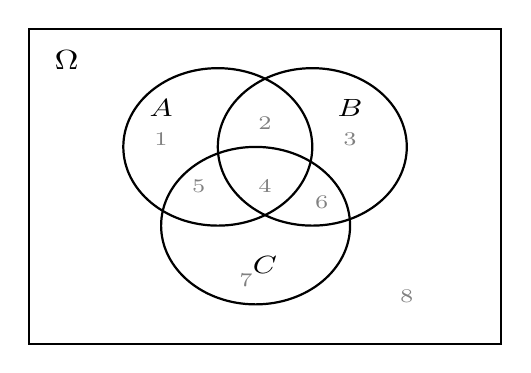
\begin{tikzpicture}[xscale=1.2, transform shape]
        \coordinate (A) at (0,0); 
        \coordinate (B) at (5,-4); 
        \coordinate (C1) at (2,-1.5);
        \coordinate (C2) at (3,-1.5);
        \coordinate (C3) at (2.4,-2.5);

        %drawing the square
        \draw[thick,thick] (A) rectangle (B);
        \foreach \C in {1,2,3}{
        \draw[thick](C\C) circle (1cm);}

        \node at (0.4, -0.4) {$\Omega$};
        \node at (1.4, -1) {\small\alert{$A$}};
        \node at (3.4, -1) {\small \alert{$B$}};
        \node at (2.5, -3) {\small \alert{$C$}};

        % nodes
        \node[gray] at (1.4,-1.4) {\scriptsize 1};
        \node[gray] at (2.5,-1.2) {\scriptsize 2};
        \node[gray] at (3.4,-1.4) {\scriptsize 3};
        \node[gray] at (2.5,-2) {\scriptsize 4};
        \node[gray] at (1.8,-2) {\scriptsize 5};
        \node[gray] at (3.1,-2.2) {\scriptsize 6};
        \node[gray] at (2.3,-3.2) {\scriptsize 7};
        \node[gray] at (4,-3.4) {\scriptsize 8};
    \end{tikzpicture}
    \end{center}
    \caption{Diagramme de Venn}%
    \label{fig:}
    \end{figure}}
\scriptsize
   Pour chaque description décrivez  les \textbf{nombres} et la
   \alert{\textbf{description mathématiques}}  de l'évènement:
    
   \only<1-2>
   {

           \scriptsize
            Au moins deux évènements des évènements $A$,$B$, $C$ sont  réalisés

           \only<2>{
               \begin{equation*}
                   (A\cap B) \cup (B\cap C) \cup (C \cap A) \quad
                   \alert{\left\{2,4,5,6\right\}}
               \end{equation*}
           }
   }

   \only<3-4>
   {

           \scriptsize
            Au plus deux évènements des évènements $A$,$B$, $C$ sont  réalisés

           \only<4>{
               \begin{equation*}
                   (A\cap B \cap C)^c \quad
                   \alert{\left\{1,2,3,5,6,7,8\right\}}
               \end{equation*}
           }
   }

   \only<5-6>
   {

           \scriptsize
            Aucun évènements des évènements $A$,$B$, $C$ est  réalisés

           \only<6>{
               \begin{equation*}
                   (A\cup B \cup C)^c \quad
                   \alert{\left\{8\right\}}
               \end{equation*}
           }
   }

   \only<7-8>
   {

           \scriptsize
            Les trois  évènements $A$,$B$, $C$ est  réalisés

           \only<8>{
               \begin{equation*}
                   A\cap B \cap C \quad
                   \alert{\left\{4\right\}}
               \end{equation*}
           }
   }

   \only<8-10>
   {

           \scriptsize
            Un seul évènement de $A$,$B$, $C$ est  réalisé

           \only<10>{
               \begin{equation*}
                   (A \cap B^c \cap C^c) \cup (B \cap C^c \cap A^c) \cup (C \cap A^c \cap B^c)\quad
                   \alert{\left\{1,3,7\right\}}
               \end{equation*}
           }
   }

   \only<11-12>
   {

           \scriptsize
           Les évènements $A$ et $B$ sont réalisés, mais pas $C$.

           \only<12>{
               \begin{equation*}
                   (A\cap B \cap C^c)\quad
                   \alert{\left\{2\right\}}
               \end{equation*}
           }
   }
\end{frame}
% }}} Vein Diagramm %

% Operation Ensemble {{{ %
\section{Probabilités et Ensembles}

\begin{frame}[<+->]
    \frametitle{Probabilités et Ensembles}
    
    \begin{itemize}
        \scriptsize
        \item  Dans cet exercice, on se propose de calculer la probabilité de 
            \begin{equation}
                \mathbf{P}(A\cup(B^c\cup C^c)^c)
            \end{equation}
            pour plusieurs cas:
        \begin{itemize}
            \scriptsize
            \item Les évènements $A$, $B$ et $C$ sont \textbf{disjoints} et
                \alert{$\mathbf{P}(A) = \frac{2}{5}$}
                \pause
                \begin{equation}
                    \scriptsize
                \end{equation}
            \item Les évènements  $A$ et $C$ sont disjoints. $P(A) =\frac{1}{2}$
                et $P(B\cap C) = \frac{1}{4}$.
                \begin{equation}
                    \scriptsize
                \end{equation}

            \item La probabilité $P(A^c \cap(B^c\cup C^c)^c) = 0.7$

                \begin{equation}
                    \scriptsize
                \end{equation}
        \end{itemize}
    \end{itemize}
\end{frame}
% }}} Operation Ensemble %

% Lance de trois coins {{{ %
\section{Lance de trois pièce de monnaie}
\begin{frame}[<+->]
    \frametitle{Trois lancés d'une pièce de monnaie}
    Vous Lancez un pièce de monnaie (H et T avec une probabilité
    $\frac{1}{2}$.\\[10pt]
    
    Pour chaque cas, calculer la probabilité des évènements suivants:\\[10pt]
    \begin{enumerate}
        \small
        \item La séquence  $\left\{H,H,H\right\}$\\[10pt]
        \item La séquence  $\left\{H,T,H\right\}$\\[10pt]
        \item Une séquence qui contient deux $H$ et un $T$.\\[10pt]
        \item Une séquence ou le nombre de $H$ est \alert{\textbf{supérieur}}
            au nombre de $T$.
    \end{enumerate}
\alert{trois fois}.
    
\end{frame}
% }}} Lance de trois coins %

% Loi uniforme dans un carre {{{ %
%{{{ premier slide
\section{Loi uniforme dans un carré}
\begin{frame}[t]
    \frametitle{Loi uniforme dans un carré}
    
    \begin{block}{Problème}
       \tiny Omar et Reda on décide de prendre un café ensemble a un temps
       précis. Les deux peuvent arriver au café avec une marge de retard
       d'\alert{\textbf{une heure}}. Tous les retards sont équiprobables (loi
       uniforme).
       \vspace*{10pt}
       \begin{itemize}
           \item Le premier qui arrive ne peut attendre que \alert{\textbf{15
               min}} avant de quitter le café.
       \end{itemize}
       \vspace*{10pt}
       Quelle est la probabilité qu'Omar et Reda prennent un café ensemble.
    \end{block}
    \begin{itemize}
        \scriptsize
        \item Espace d'états (Simplification):
            \begin{equation*}
               \Omega = \left\{\left(\frac{i}{4}, \frac{j}{4}\right)\;|\; (i,j) \in
                   \{1,2,3,4\}\right\} 
            \end{equation*}
    \end{itemize}
    \begin{figure}[htpb]
    \begin{center}
    \begin{tikzpicture}[scale=0.5, transform shape]
        
        \foreach \x in {0,1,2,3,4}
        {
            \foreach \y in {0,1,2,3,4}
        {
            \node[draw,inner sep=0pt, minimum width=2pt,circle,fill] at (\x,\y) {};
        }
        \node[sexyRed]at (\x, -1) {$\x/4$};
        \node[sexyRed]at (-1, \x) {$\x/4$};
        }
        \node[] at (2.5,-2) {\textbf{Omar}};
        \node[rotate=90] at (-2,2.5) {\textbf{Reda}};
        \node[draw,sexyRed, inner sep=0pt, minimum width=8pt,rectangle,minimum
            height=8pt ] at (1,2){};

     \only<2->
     {
        \node[draw,sexyRed, inner sep=0pt, minimum width=8pt,rectangle,minimum
            height=8pt ] at (3,4){};
        \node[draw,sexyRed, inner sep=0pt, minimum width=8pt,rectangle,minimum
            height=8pt ] at (4,4){};
        \node[draw,sexyRed, inner sep=0pt, minimum width=8pt,rectangle,minimum
            height=8pt ] at (4,3){};

        \node[draw,sexyRed, inner sep=0pt, minimum width=8pt,rectangle,minimum
            height=8pt ] at (3,3){};

        \node[draw,sexyRed, inner sep=0pt, minimum width=8pt,rectangle,minimum
            height=8pt ] at (2,3){};

        \node[draw,sexyRed, inner sep=0pt, minimum width=8pt,rectangle,minimum
            height=8pt ] at (3,2){};

        \node[draw,sexyRed, inner sep=0pt, minimum width=8pt,rectangle,minimum
            height=8pt ] at (2,2){};

        \node[draw,sexyRed, inner sep=0pt, minimum width=8pt,rectangle,minimum
            height=8pt ] at (1,2){};

        \node[draw,sexyRed, inner sep=0pt, minimum width=8pt,rectangle,minimum
            height=8pt ] at (2,1){};

        \node[draw,sexyRed, inner sep=0pt, minimum width=8pt,rectangle,minimum
            height=8pt ] at (1,1){};

        \node[draw,sexyRed, inner sep=0pt, minimum width=8pt,rectangle,minimum
            height=8pt ] at (0,1){};

        \node[draw,sexyRed, inner sep=0pt, minimum width=8pt,rectangle,minimum
            height=8pt ] at (0,0){};

        \node[draw,sexyRed, inner sep=0pt, minimum width=8pt,rectangle,minimum
            height=8pt ] at (1,0){};
     }

    \end{tikzpicture}
    \end{center}
    \end{figure}
    
\end{frame}
%}}}

%{{{ Deuxieme slide
\begin{frame}[t]
    \frametitle{Loi uniforme dans un carré}
    
    \begin{itemize}
        \scriptsize
        \item Espace d'états :
            \begin{equation*}
               \Omega = \left\{\left(x, y\right)\;|\; (x,y) \in
                   \left[0,1\right]\right\} 
            \end{equation*}
    \end{itemize}
    \begin{figure}[htpb]
    \begin{center}
    \begin{tikzpicture}[scale=0.6, transform shape]
        
        \foreach \x in {0,1,2,3,4}
        {
            \foreach \y in {0,1,2,3,4}
        {
            \node[draw,inner sep=0pt, minimum width=2pt,circle,fill] at (\x,\y) {};
        }
        \draw[thick,opacity=0.5,lightgray] (0,0) rectangle (4,4);
        \node[sexyRed]at (\x, -1) {$\x/4$};
        \node[sexyRed]at (-1, \x) {$\x/4$};
        }
        \node[] at (2.5,-2) {\textbf{Omar}};
        \node[rotate=90] at (-2,2.5) {\textbf{Reda}};
        \node[draw,sexyRed, inner sep=0pt, minimum width=8pt,rectangle,minimum
            height=8pt ] at (1,2){};

     \only<1->
     {
        \node[draw,sexyRed, inner sep=0pt, minimum width=8pt,rectangle,minimum
            height=8pt ] at (3,4){};
        \node[draw,sexyRed, inner sep=0pt, minimum width=8pt,rectangle,minimum
            height=8pt ] at (4,4){};
        \node[draw,sexyRed, inner sep=0pt, minimum width=8pt,rectangle,minimum
            height=8pt ] at (4,3){};

        \node[draw,sexyRed, inner sep=0pt, minimum width=8pt,rectangle,minimum
            height=8pt ] at (3,3){};

        \node[draw,sexyRed, inner sep=0pt, minimum width=8pt,rectangle,minimum
            height=8pt ] at (2,3){};

        \node[draw,sexyRed, inner sep=0pt, minimum width=8pt,rectangle,minimum
            height=8pt ] at (3,2){};

        \node[draw,sexyRed, inner sep=0pt, minimum width=8pt,rectangle,minimum
            height=8pt ] at (2,2){};

        \node[draw,sexyRed, inner sep=0pt, minimum width=8pt,rectangle,minimum
            height=8pt ] at (1,2){};

        \node[draw,sexyRed, inner sep=0pt, minimum width=8pt,rectangle,minimum
            height=8pt ] at (2,1){};

        \node[draw,sexyRed, inner sep=0pt, minimum width=8pt,rectangle,minimum
            height=8pt ] at (1,1){};

        \node[draw,sexyRed, inner sep=0pt, minimum width=8pt,rectangle,minimum
            height=8pt ] at (0,1){};

        \node[draw,sexyRed, inner sep=0pt, minimum width=8pt,rectangle,minimum
            height=8pt ] at (0,0){};

        \node[draw,sexyRed, inner sep=0pt, minimum width=8pt,rectangle,minimum
            height=8pt ] at (1,0){};
     }
     \only<2->
     {
         \fill[sexyRed,opacity=0.4](0,0) -- (0,1) -- (3,4)--(4,4)--(4,3)--(1,0)--cycle;
     }

    \end{tikzpicture}
    \end{center}
    \end{figure}
    \only<3->
    {
    
    \begin{equation}
        \mathbf{P}(A) = 1 -
        2*\left(\frac{1}{2}\times\frac{3}{4}\times\frac{3}{4}\right) =
        \frac{7}{16}
    \end{equation}
}
\end{frame}
%}}}
% }}} Loi uniforme dans un carre %

\end{document}
